\renewcommand{\theequation}{\theenumi}
%\subsection{Problem}

\begin{enumerate}[label=\arabic*.,ref=\thesubsection.\theenumi]
\numberwithin{equation}{enumi}
%
%
\item Consider the optimization problem
\begin{align}
\label{eq:opt_def}
\max_{z} \frac{1}{\abs{z-1}}
\\
s.t. \quad \abs{z-2 + \j} \ge \sqrt{5}
\end{align}
%
Show that it can be reframed as
\begin{align}
\label{eq:opt_rev}
\min_{\vec{x}} \,\norm{\vec{x} - \vec{c}_1}^2
\\
 s.t. \quad  \norm{\vec{x} - \vec{c}_2}^2 \ge 5
%\min_{z} \abs{z-1}
%\\
% s.t. \quad \abs{z-2 + \j} \ge \sqrt{5}
\end{align}
%
where
\begin{align}
z &= \vec{x} = \myvec{x_1 \\ x_2},
%\\
\vec{c}_1 = \myvec{1 \\ 0},
%\\
\vec{c}_2 = \myvec{2 \\ -1}
\end{align}

%
%
%Then, 
%\begin{align}
%\Gamma: \abs{z-1} = \norm{\vec{x} - \vec{c}_1}^2,
%\end{align}
%where 
%\begin{align}
%\end{align}
%Similarly, 
%\begin{align}
%\Omega:\abs{z-2+\j} = \norm{\vec{x} - \vec{c}_2}^2,
%\end{align}
%where 
%\begin{align}
%\end{align}
%
%Let 
%\begin{align}
% \abs{z_0-1} = r
%\end{align}
%
%
\item Explain the optimization problem with a figure.
\\
\solution
Fig. \ref{fig:2019_1} explains \eqref{eq:opt_rev}
where $z_0$ is the set of points comprising of the intersection of the 
smallest circle $\Gamma:$ with the largest circle $\Omega: r_2 \ge 
\sqrt{5}$ 
with radii 
$r_1$ and 
$r_2 \ge \sqrt{5}$ respectively.
\begin{figure}[!ht]
\centering
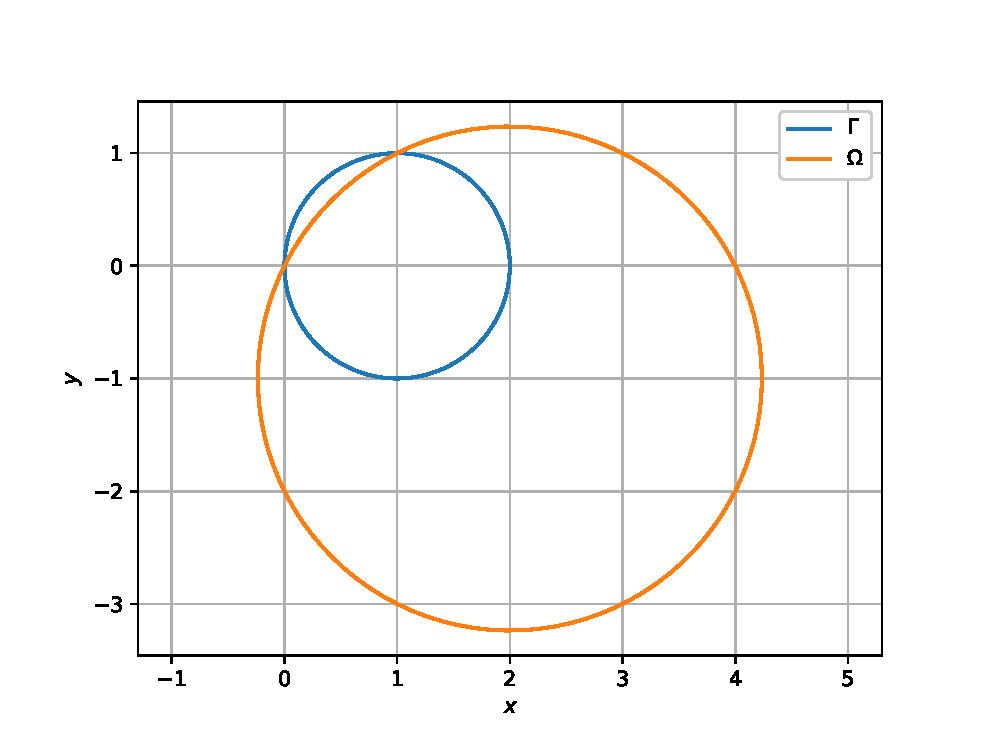
\includegraphics[width=\columnwidth]{./optimization/figs/2019_1_1.eps}
\caption{}
\label{fig:2019_1}
\end{figure}
%
\item Obtain the Lagrangian.
\\
\solution
The Lagrangian is 
\begin{align}
L \brak{\vec{x},\lambda} = \norm{\vec{x} - \vec{c}_1}^2 - \lambda 
\cbrak{\norm{\vec{x} - \vec{c}_2}^2-r_2^2}
\end{align}
\item Use the KKT conditions to obtain the minima.
\\
\solution
From the KKT conditions, 
\begin{align}
\frac{\partial L \brak{\vec{x},\lambda}}{\partial \vec{x}} &= 0
\\
\implies {\vec{x} - \vec{c}_1} - \lambda \brak{\vec{x} - \vec{c}_2} &= 0
\\
\implies \vec{x}  = \frac{\vec{c}_1 -\lambda  \vec{c}_2}{1-\lambda } &
\label{eq:opt_xlam}
\end{align}
%
and 
\begin{align}
\frac{\partial L \brak{\vec{x},\lambda}}{\partial \lambda} &= 0
\\
\implies \norm{\vec{x} - \vec{c}_2}^2-r_2^2 &= 0
\label{eq:opt_xnorm}
\end{align}
Substituting from \eqref{eq:opt_xlam} in \eqref{eq:opt_xnorm},
\begin{align}
\norm{\frac{\vec{c}_1 -\lambda  \vec{c}_2}{1-\lambda } - \vec{c}_2}^2-r_2^2 &= 0
\\
\implies \lambda = 1\pm \frac{\norm{\vec{c}_1 - \vec{c}_2}}{r_2}&
\\
= 1 \pm \sqrt{\frac{2}{5}}
%\label{eq:opt_xnorm}
\end{align}
Fig. \ref{fig:2019_1_2} plots $\Gamma$ for 
\begin{align}
\lambda = 1 - \sqrt{\frac{2}{5}}
\end{align}
\item If the maximum value is obtained at $z_0$, find the principal argument of
\begin{align}
\frac{4 - z_0-\bar{z}_0}{z_0-\bar{z}_0+2\j}
\end{align}
\\
\solution 
From \eqref{eq:opt_xlam},
\begin{align}
 \vec{x}_0  &= \frac{\vec{c}_1 -\lambda  \vec{c}_2}{1-\lambda } 
\\
\implies z_0 &= \frac{1}{1-\lambda}\brak{1-2\lambda + \j \lambda }
\\
\text{or, }\arg \frac{4 - z_0-\bar{z}_0}{z_0-\bar{z}_0+2\j} &= \frac{2 - \Re\cbrak{z_0}}{\j\brak{\Im\cbrak{z_0}+1}}
\\
&=\frac{2\brak{1-\lambda}-\brak{1-2\lambda}}{\j} 
\\
&= -\j
\end{align}
%
Thus, the principal argument is $-\frac{\pi}{2}$.
\begin{figure}[!ht]
\centering
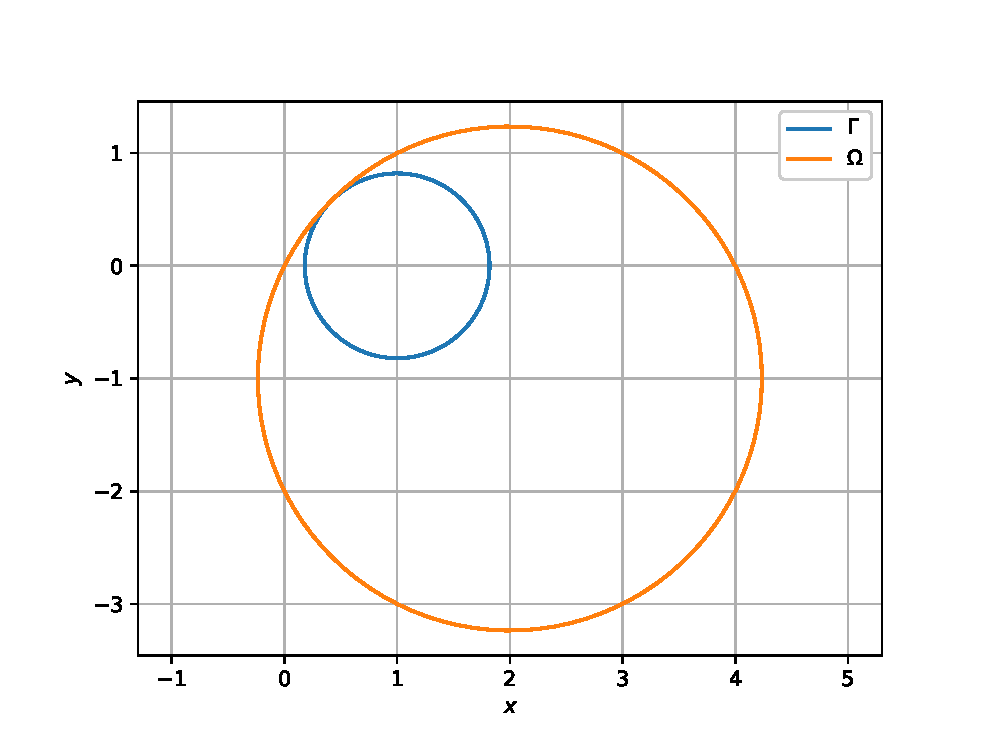
\includegraphics[width=\columnwidth]{./optimization/figs/2019_1_2.eps}
\caption{}
\label{fig:2019_1_2}
\end{figure}

%\begin{enumerate}[label=\theenumi.\arabic*
%,ref=\thesection.\theenumi]
\item Show that the set 
\begin{align}
D = \cbrak{\vec{x}:\norm{\vec{x}-\vec{C}_2} \ge r_2}, r_2 > 0
\end{align}
%
is nonconvex.
\\
\solution Let $\vec{x}_1 \in D$ and 
\begin{align}
\vec{x}_2 = 2\vec{C}_2-\vec{x}_1
\end{align}
Then 
\begin{align}
\norm{\vec{x}_2-\vec{C}_2} &= \norm{\vec{C}_2-\vec{x}_1} \ge r_2
\\
\implies \vec{x}_2 &\in D.
\end{align}
Suppose 
\begin{align}
\vec{x} = \theta\vec{x}_1+\brak{1-\theta}\vec{x}_2
\end{align}
For $\theta = \frac{1}{2}$,
\begin{align}
\vec{x} &= \vec{C}_2
\\
\implies \norm{\vec{x}-\vec{C}_2} &= 0,
\\
\text{or, } \vec{x} &\notin D
\end{align}
Thus, by definition, $D$ is not a convex set.
\end{enumerate}


